Grafičko sučelje predstavlja prikladan način za korisnika kako bi jednostavno obavljao zadatke upravljanja karticama
i pregleda dnevnika pristupa.
Prethodno definirane funkcionalnosti u pozadinskoj aplikaciji koje treba implementirati u grafičkom sučelju su:

\begin{itemize}
    \item Autorizacija korisnika
    \item Upravljanje karticama
    \item Pregled dnevnika pristupa
\end{itemize}

Aplikacije na web platformi koje se izvršavaju u pregledniku nemaju mogućnost odabira jezika.
Tri su jezika potrebna za izradu grafičkog sučelja na web platformi: HTML, CSS i JavaScript.
Pri razvoju sučelja koristi se radni okvir \textit{Vue}, a osnovne vizualne komponente pruža \textit{Vuetify}.

\subsection{Autorizacija korisnika}

Prije poduzimanja bilo kojih akcija, korisnik se mora autorizirati (prijaviti) u aplikaciju.
Forma za unos pristupnih podataka prikazana je u nastavku.

\begin{figure}[h!]
    \centering
    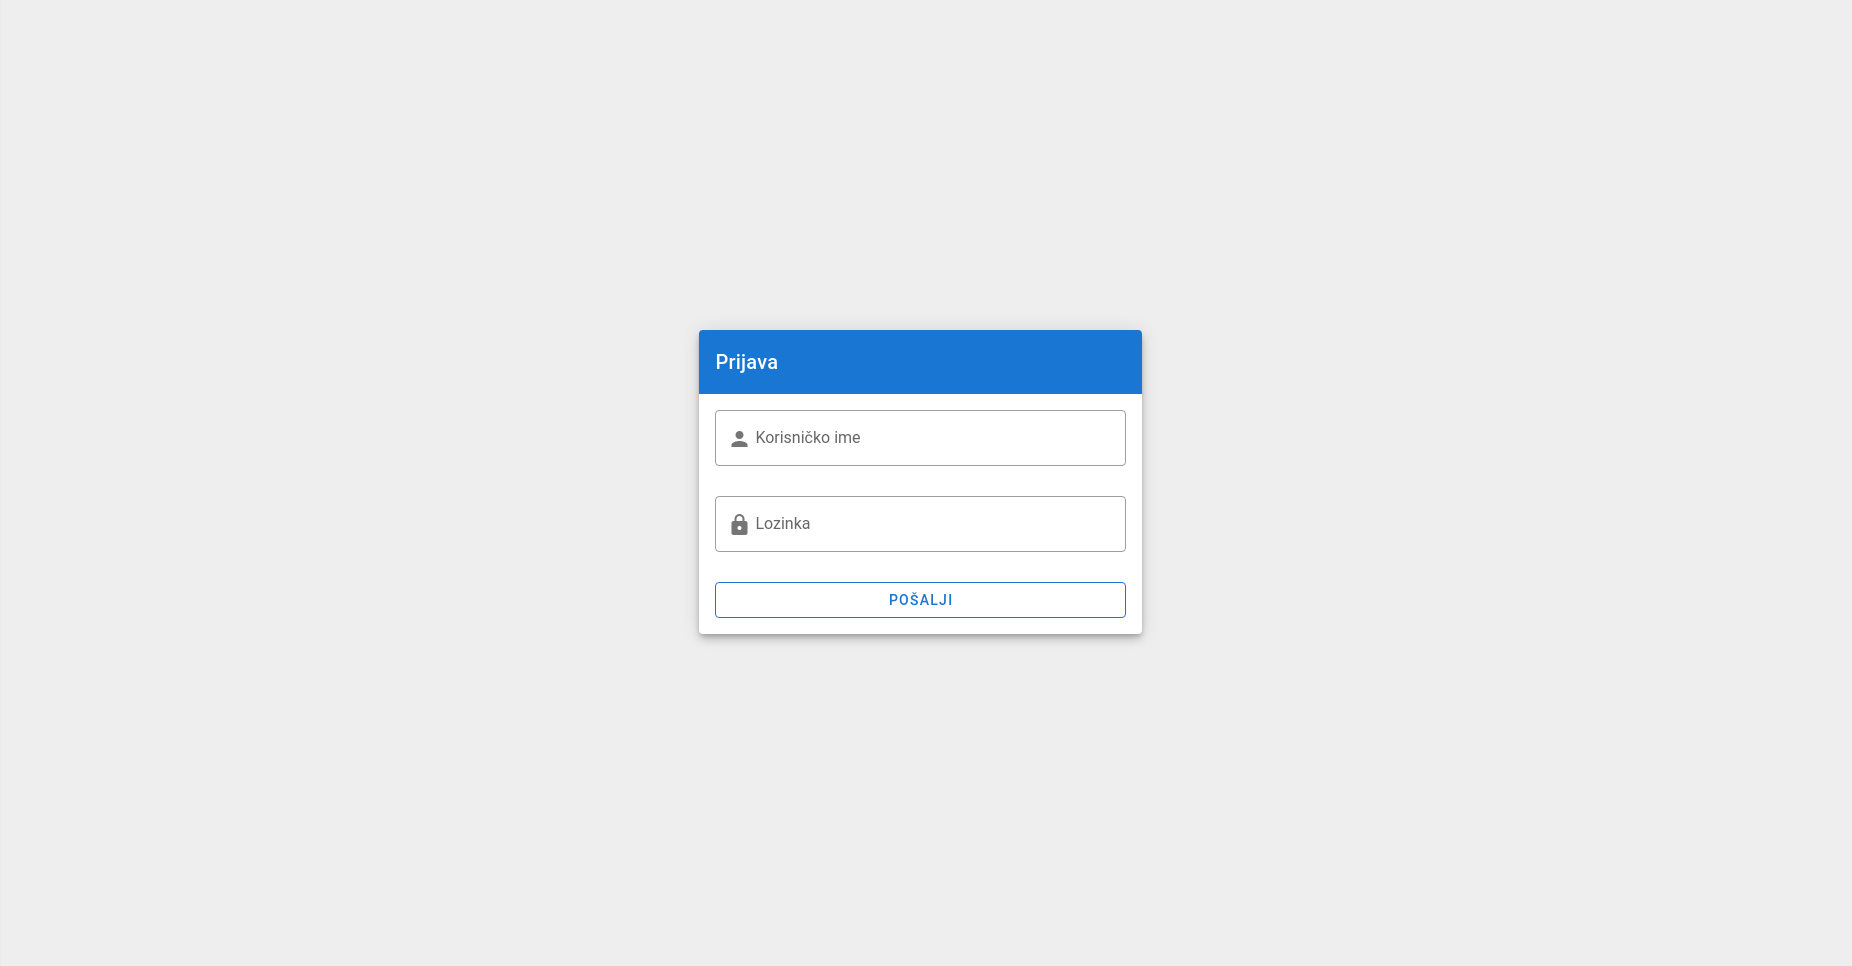
\includegraphics[width=\textwidth]{images/login-view}
    \caption{Forma za unos pristupnih podataka}
    \label{fig:login-view}
\end{figure}

\pagebreak

Na slici~\ref{fig:login-view} su tri važne komponente za obavljanje autorizacije:

\begin{enumerate}
    \item Polje za unos korisničkog imena
        \begin{lstlisting}[language=HTML]
<v-text-field
    v-model="username.value"
    label="Korisnicko ime"
    prepend-inner-icon="mdi-account"
    outlined
/>
        \end{lstlisting}
    \item Polje za unos lozinke
        \begin{lstlisting}[language=HTML]
<v-text-field
    v-model="password.value"
    type="password"
    label="Lozinka"
    prepend-inner-icon="mdi-lock"
    outlined
/>
        \end{lstlisting}
    \item Gumb za slanje zahtjeva
        \begin{lstlisting}[language=HTML]
<v-btn
    color="primary"
    type="submit"
    block
    outlined
>
    Posalji
</v-btn>
        \end{lstlisting}
\end{enumerate}

Komponente su omotane oko \textit{v-form} komponente koja je zaslužna za slanje zahtjeva kad korisnik pritisne gumb.

\begin{lstlisting}[language=HTML]
<v-form @submit.prevent="login">
</v-form>
\end{lstlisting}

Kako HTML ne može slati zahtjeve prema serveru i izvoditi bilo kakvu logiku, funkcija \textit{login} koja se okida na
\textit{submit} događaj je implementirana pomoću JavaScript jezika.

\begin{lstlisting}
import axios from 'axios'

export default {
  name: 'LoginForm',

  data: () => ({
    username: {
      value: ''
    },
    password: {
      value: ''
    }
  }),

  methods: {
    async login () {
      const { data } = await axios.post('/api/login', { username: this.username.value, password: this.password.value })
      const serverResponse = data.data

      this.loginSuccessful(serverResponse)
    },

    loginSuccessful (messageForUser) {
      this.$emit('success', messageForUser)
    }
  }
}
\end{lstlisting}

Svaka komponenta ima naziv \textbf{name}, može sadržavati podatke \textbf{data}, implementirati metode \textbf{methods} i sl.
U funkciji \textit{data} se nalazi objekt s vrijednostima polja koja korisnik mora ispuniti.
U \textit{methods} objektu je jedna metoda \textbf{login} koja je zadužena za slanje zahtjeva na pozadinsku aplikaciju.
Koristi se biblioteka \textbf{axios} jer olakšava slanje zahtjeva naspram standardnih \textit{fetch} i \textit{XMLHttpRequest} funkcija.
Nakon uspješne autorizacije metoda \textit{\$emit} emitira događaj i obavještava nadređenu komponentu.
Tada nadređena komponenta zna da može učitati pristupni dnevnik i kartice.

\begin{figure}[h!]
    \centering
    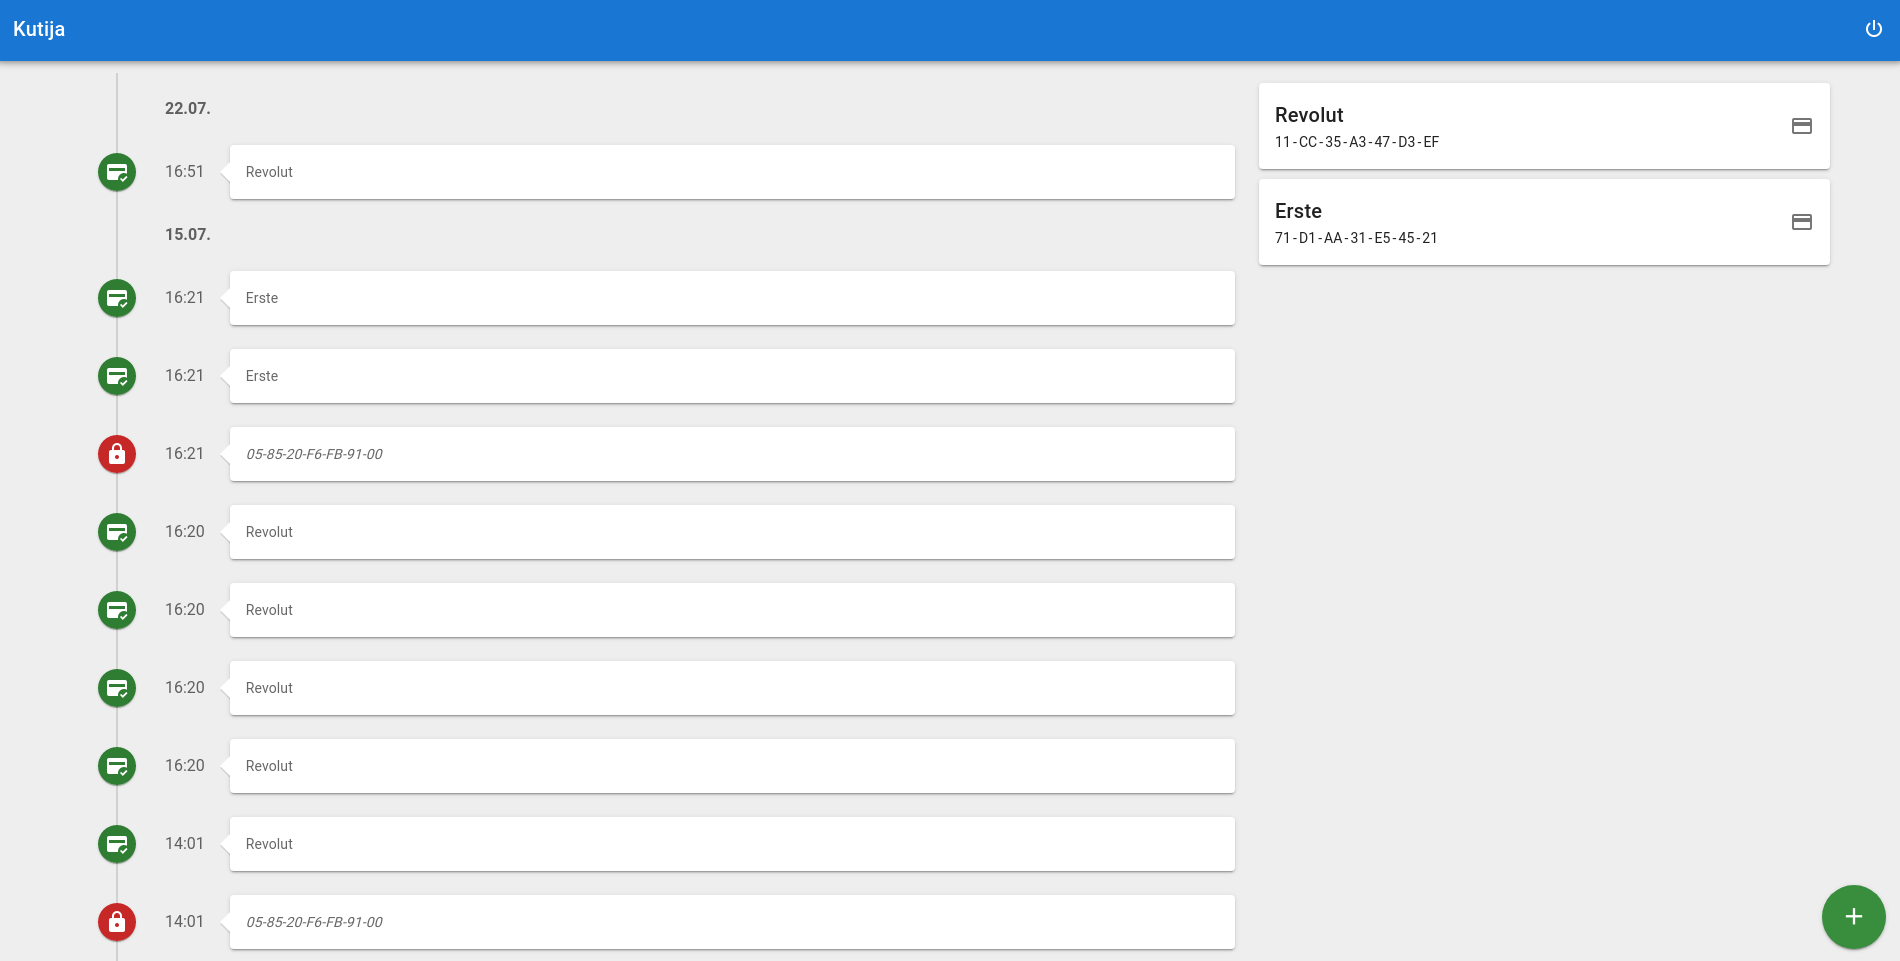
\includegraphics[width=\textwidth]{images/primary-view}
    \caption{Pristupni dnevnik i kartice}
\end{figure}

\pagebreak

\subsection{Upravljanje karticama}

Za prikaz svih kartica potrebne su dvije komponente: komponenta za dohvaćanje kartica sa servera i komponenta za prikaz
istih.

\begin{lstlisting}[language=HTML]
<CardListData>
  <template v-slot:default="{ cards, addCard, removeCard, updateCard }">
    <CardList
      :cards="cards"
      @card-created="addCard"
      @card-deleted="removeCard"
      @card-updated="updateCard"
    />
  </template>
</CardListData>
\end{lstlisting}

Komponenta \textbf{CardListData} se brine o načinu dohvaćanja podataka, sprema ih u varijablu \textit{cards} kao polje
s podacima kartica.

Kako je kartice moguće uređivati, brisati i dodavati nije prikladno da komponenta koja konzumira varijablu \textit{cards}
ujedno i izmjenjuje istu.
Kako bi pravilno napravila izmjene, komponenta \textbf{CardList} mora znati unutarnje ponašanje komponente \textbf{CardListData}.
To dovodi do curenja apstrakcije (eng. \textit{abstraction leak}) pa iz tog razloga postoje tri metode:
\textit{addCard}, \textit{removeCard}, \textit{updateCard}.
Na taj način komponenta \textit{CardListData} pruža stabilan API. Komponenta \textit{CardList} mora znati potrebne argumente
za svaku funkciju, a ne mora znati na koji način će se promjene izvesti.

Komponenta \textbf{CardList} pomoću petlje jednostavno prikazuje sve kartice.
Kako je svaku karticu moguće mijenjati i brisati potrebna je dodatna komponenta: \textbf{CardListItem}.
Ona zahtjeva naziv i UID kartice, a ima tri stanja u kojima se može nalaziti:

\begin{enumerate}
    \item Zadano stanje - samo prikazuje naziv i UID te gumbe za uređivanje ili brisanje
    \item Stanje uređivanja - polje za unos naziva i gumb za spremanje ili odustajanje
    \item Stanje brisanja - gumb za potvrdu brisanja i gumb za odustajanje
\end{enumerate}

\pagebreak

\begin{figure}[h!]
    \centering
    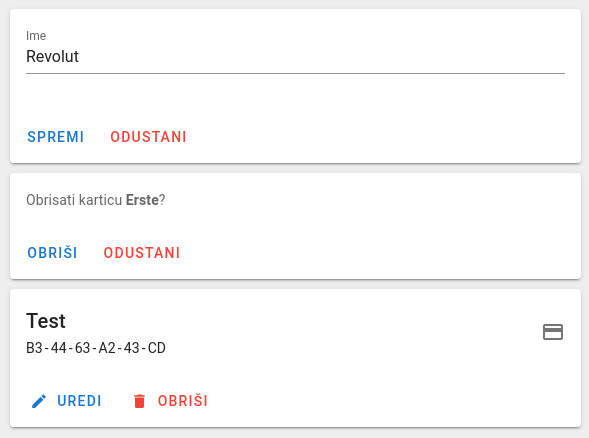
\includegraphics[scale=0.5]{images/card-states}
    \caption{Tri stanja kartice}
    \label{fig:card-states}
\end{figure}

Na slici~\ref{fig:card-states} prva kartica je u stanju uređivanja, druga je u stanju brisanja, a posljednja je u zadanom
stanju.
Iako u programskom kodu nije eksplicitno definirana, postoji implicitna mašina stanja (eng. \textit{state machine}).
Mašina stanja je koncept ponašanja programa definiran kroz konačan broj stanja i tranzicija.
Svako stanje pruža relevantne informacije o programu, dok tranzicije ukazuju na moguće prijelaze između stanja~\cite{state-machine}.
Jedna od prednosti mašine stanja je mogućnost kreiranja dijagrama stanja i prijelaza.

\begin{figure}[h!]
    \centering
    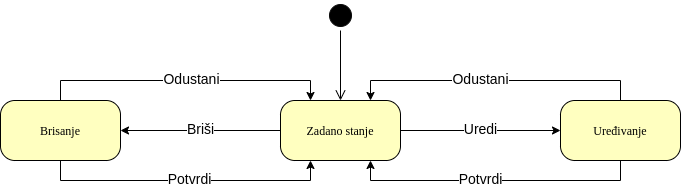
\includegraphics[scale=0.5]{images/card-state-machine}
    \caption{Tri stanja kartice}
    \label{fig:card-state-machine}
\end{figure}

Na slici~\ref{fig:card-state-machine} prikazan je dijagram mašine stanja jedne kartice.
Zadano stanje je ujedno i početno stanje (eng. \textit{initial state}) i jedino iz tog stanja se može prijeći
u druga dva uz pomoć tranzicija "Briši" i "Uredi".
Druga dva stanja imaju po dvije tranzicije "Potvrdi" i "Odustani" koje vode u zadano stanje.
Prema dijagramu nije moguće direktno prijeći iz stanja brisanja u stanje uređivanja.

Svako stanje zahtjeva nešto drugačije sučelje i elemente pa je pogodno kreirati zasebne komponente za svako stanje.
Tri su komponente potrebne:
\begin{enumerate}
    \item \textbf{CardListItemDefaultState}
    \item \textbf{CardListItemEditState}
    \item \textbf{CardListItemDeleteState}
\end{enumerate}

Sve tri komponente su omotane oko komponente \textbf{CardListItem}.
Ona se brine o trenutnom stanju kao i o prelasku u druga stanja pa je to čini "mašinom" u mašini stanja.

\begin{lstlisting}[language=HTML]
<CardItemEditState
    v-if="inEditMode"

    :id="id"
    :name="name"

    @cancel="stopEdit"
    @success="completeEdit"
/>
<CardItemDeleteState
    v-else-if="inDeleteMode"

    :id="id"
    :name="name"

    @cancel="stopDelete"
    @success="completeDelete"
/>
<CardItemDefaultState
    v-else

    :name="name"
    :uid="uid"

    @edit-requested="startEdit"
    @delete-requested="startDelete"
/>
\end{lstlisting}

Direktive \textit{v-if}, \textit{v-else-if}, \textit{v-else} se brinu da u jednom trenutku korisniku bude vidljiva samo
jedna komponenta (jedno stanje).
Na događaje (\textit{@success}, \textit{@cancel}, \ldots) izvršavaju se metode (\textit{startEdit}, \textit{stopDelete}, \ldots)
i one predstavljaju tranzicije - prelazak iz jednog stanja u drugi.

\begin{lstlisting}
data: () => ({
    editActive: false
}),

computed: {
    inEditMode () {
      return this.editActive === true
    },
},

methods: {
    startEdit () {
      this.editActive = true
    },

    stopEdit () {
      this.editActive = false
    }
}
\end{lstlisting}

Sve tri komponente su trivijalne - uglavnom definiraju izgled i nemaju previše logike.
Važno je naglasiti da u komponenti \textit{CardListItemEditState} kad korisnik klikne na gumb "Spremi" šalje se zahtjev
na pozadinsku aplikaciju koji ažurira naziv kartice.

\begin{lstlisting}
axios.put('/api/card/' + this.id, { name: this.newName.value })
\end{lstlisting}

Slična je situacija i s \textit{CardListItemDeleteState} komponentom.
Kada korisnik klikne na gumb "Obriši" šalje se zahtjev na pozadinsku aplikaciju koji briše karticu.

\begin{lstlisting}
axios.delete('/api/card/' + this.id)
\end{lstlisting}

Preostalo je implementirati dodavanje novih kartica.

\begin{figure}[h!]
    \centering
    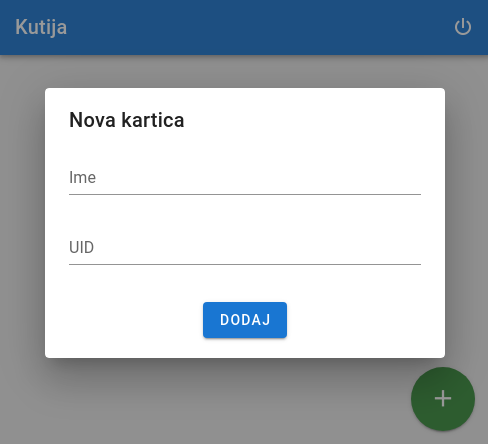
\includegraphics[scale=0.5]{images/add-new-card}
    \caption{Dodavanje nove kartice}
    \label{fig:new-card-window}
\end{figure}

Na slici~\ref{fig:new-card-window} prikazan je prozor s formom za unos nove kartice.
Poput forme za autorizaciju korisnika, dodavanje nove kartice ima tri važne komponente:

\begin{enumerate}
    \item Polje za unos naziva kartice
        \begin{lstlisting}[language=HTML]
<v-text-field
    v-model="name.value"

    label="Ime"
    hint="npr. Glavna kartica"
    maxlength="30"
/>
        \end{lstlisting}
    \item Polje za unos jedinstvenog identifikatora (UID)
        \begin{lstlisting}[language=HTML]
<v-text-field
    v-model="uid.value"

    label="UID"
    hint="npr. A5-C1-23-13-1C-7E"
    maxlength="40"
/>
        \end{lstlisting}
    \item Gumb za slanje zahtjeva
        \begin{lstlisting}[language=HTML]
<v-btn
    color="primary"
    type="submit"
>
    Dodaj
</v-btn>
        \end{lstlisting}
\end{enumerate}

Komponenta za slanje zahtjeva prilikom pritiska gumba:

\begin{lstlisting}[language=HTML]
<v-form @submit.prevent="submitNewCard">
</v-form>
\end{lstlisting}

Ove komponente i skripta za slanje zahtjeva čine komponentu \textbf{CardListNewItem}:

\begin{lstlisting}
export default {
  name: 'CardListNewItemForm',

  data: () => ({
    name: {
      value: ''
    },
    uid: {
      value: ''
    }
  }),

  methods: {
    async submitNewCard () {
        const { data } = await axios.post('/api/card', {
          name: this.name.value,
          uid: this.uid.value
        })

        const { id, name, uid } = data.data
        this.cardCreated({ id, name, uid })
    }
  }
}
\end{lstlisting}
